\section{Vierte Sequenz}
Nachdem nun die Kraftübertragung des Autos auf den Kranarm beschrieben und daraus eine resultierende Bewegung des Krans abgeleitet wurde, soll abschließend untersucht werden, wie die Kollision der Kugel mit dem ausschwenkenden Gegengewicht verläuft. 

\begin{wrapfigure}{l}{0.5\textwidth} %L
	\centering
	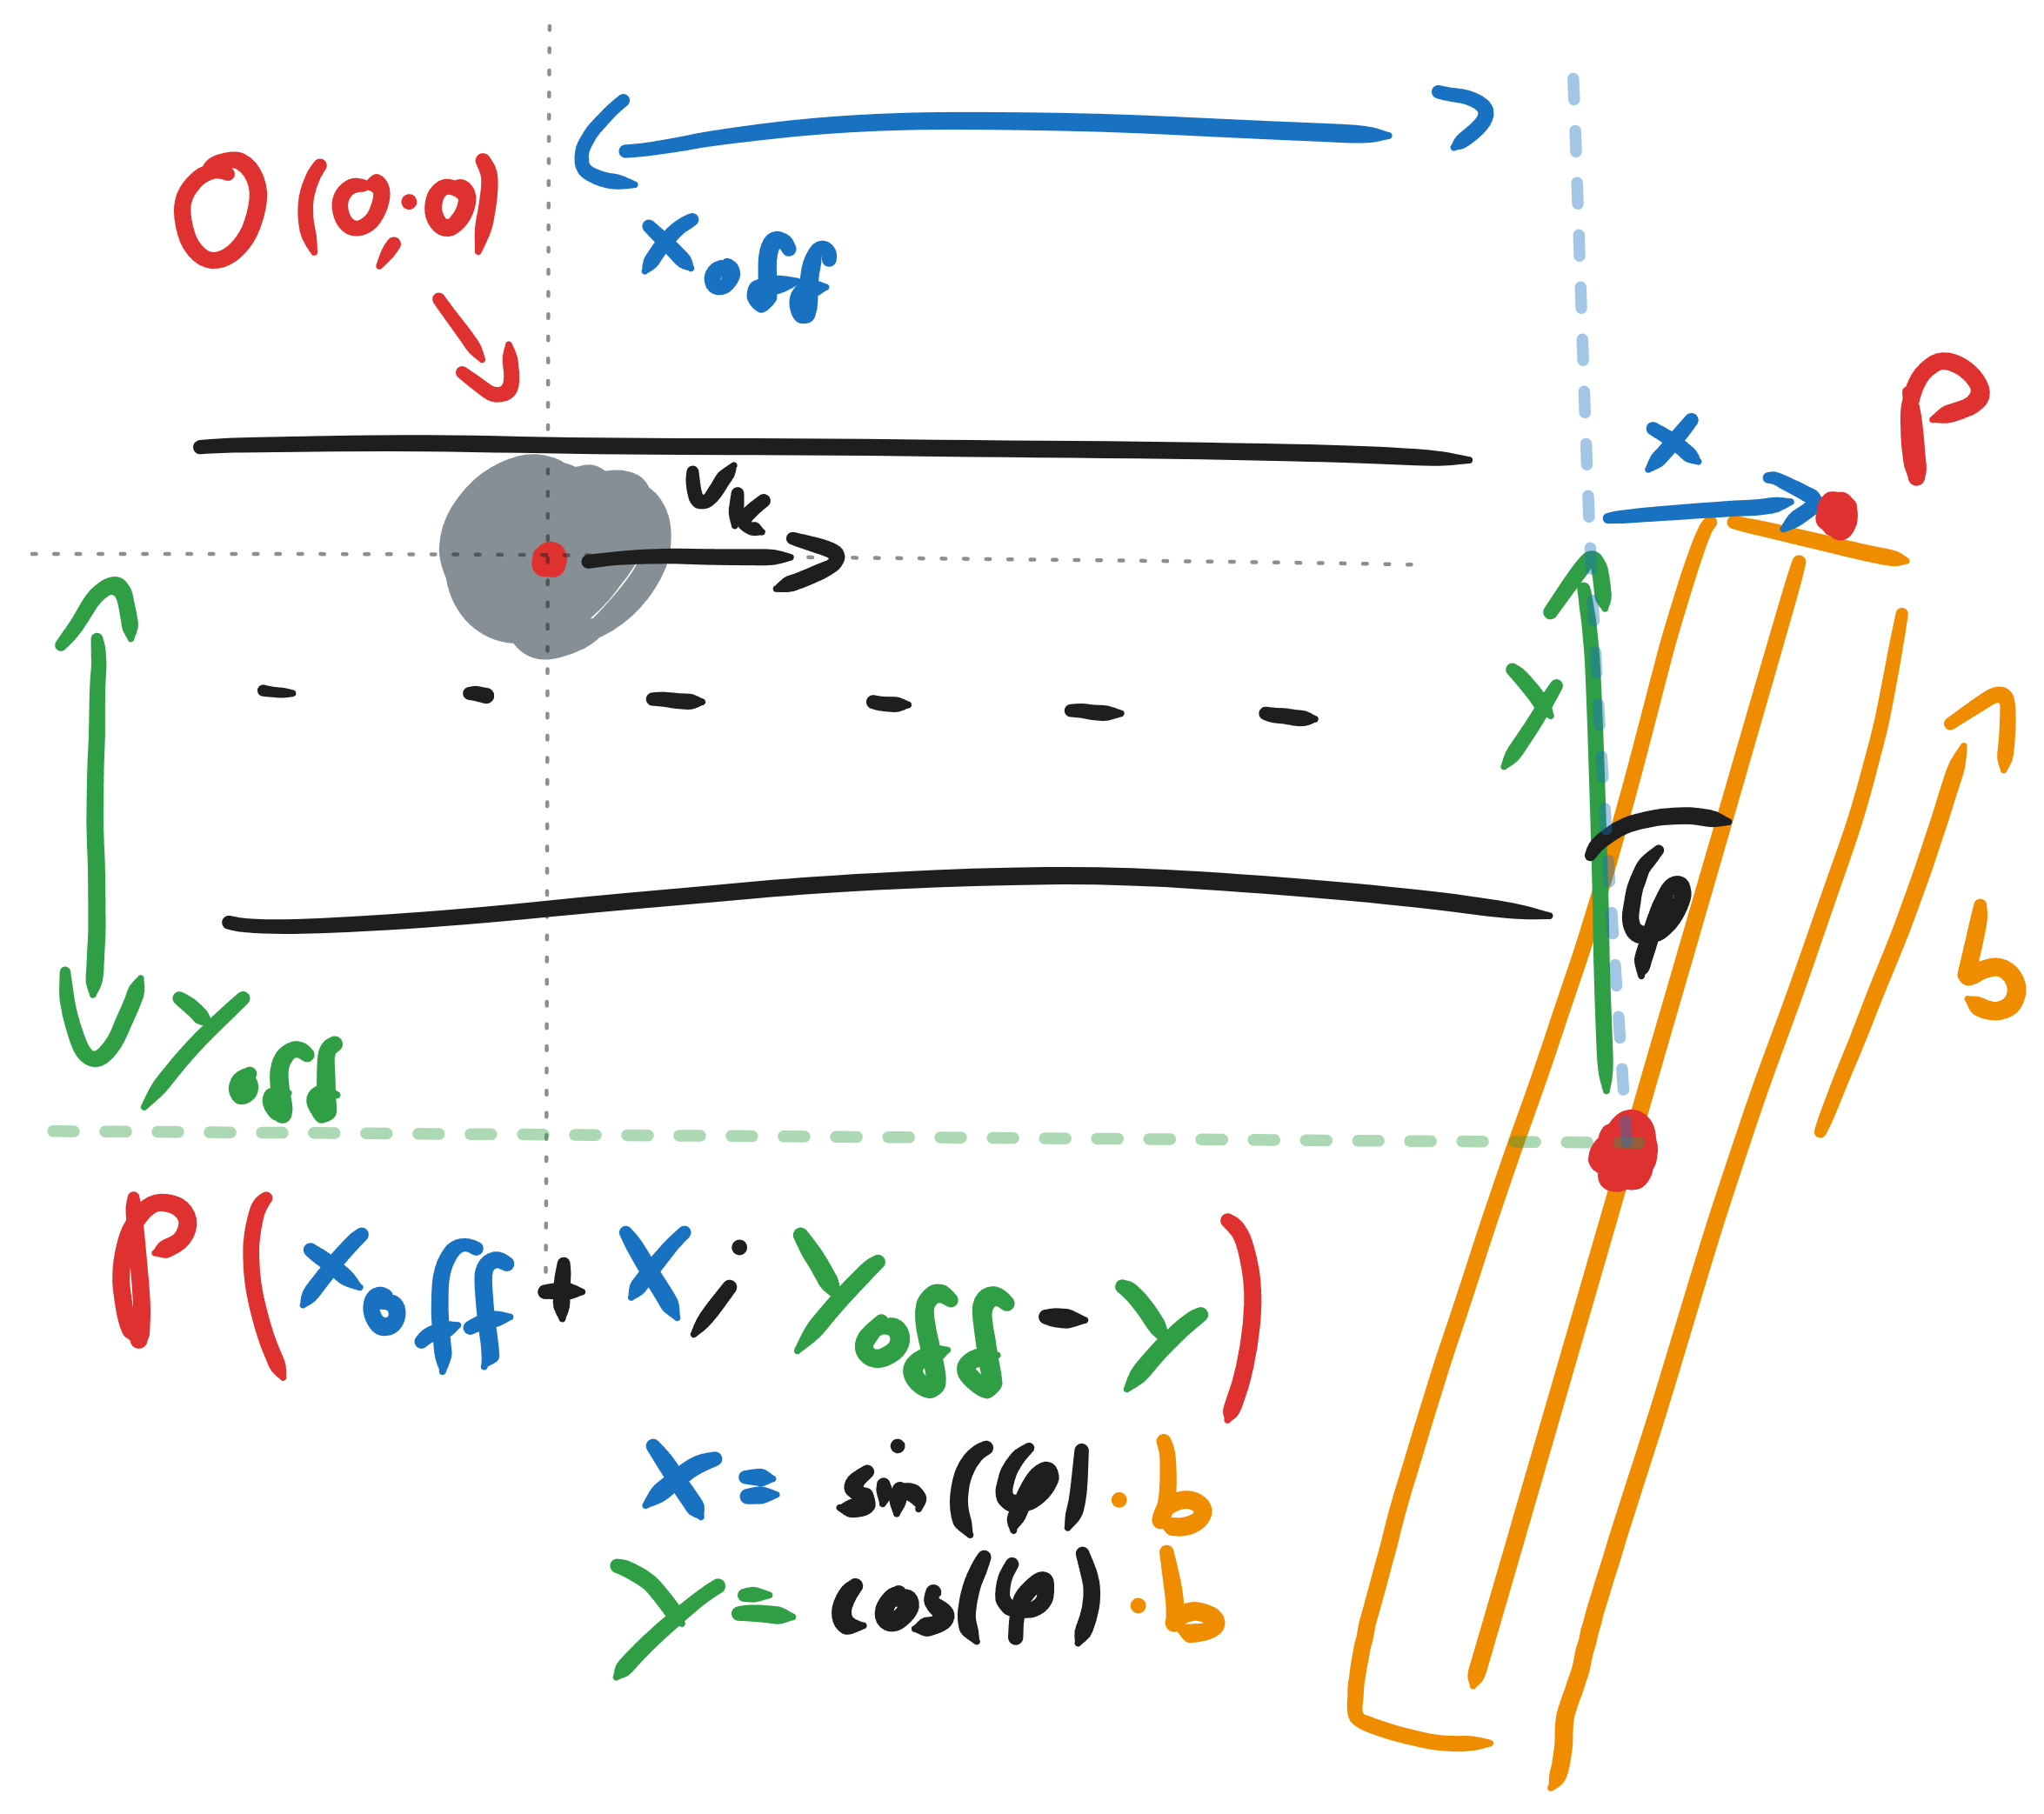
\includegraphics[width=0.48\textwidth]{resources/seq5/00_sketch-initial.png}
	\vspace*{-5mm}
	\begin{flushright}
		{\scriptsize Eigenkreation; Gezeichnet in Excalidraw}
	\end{flushright}
	
	\captionsetup{
		labelfont=bf,
		textfont=footnotesize,
		skip=0pt
	}
	\caption{Einfache Skizze der 4. Sequenz in Draufsicht}
	\label{fig:05_sketch_initial}
	%\vspace{-10pt}
\end{wrapfigure}

In \hyperref[fig:05_sketch_initial]{Abbildung~\ref*{fig:05_sketch_initial}} ist eine vereinfachte Darstellung des Szenarios zu sehen. Die Kugel rollt ausgehend vom Ursprung des imaginären Koordinatensystems und trifft den Kranarm im Punkt $P$. Sämtliche Umgebungsparameter müssen in diesem Zusammenhang neu definiert werden, da zwar ähnliche Konstellationen bereits untersucht wurden, diese jedoch auf die Position des Autos und des Kranauslegers bezogen waren – nicht jedoch auf die der Kugel und des Gegengewichts. Der Abstand des Kugelursprungs zum Krandrehpunkt, also $x_\text{off}$ und $y_\text{off}$, ist daher neu zu bestimmen; ebenso ist die Anfangsgeschwindigkeit der Kugel bislang unbekannt. Der Kranwinkel $\varphi$ zum Zeitpunkt der Kollision zwischen Kugel und Gegengewicht kann hingegen aus der zuvor ermittelten resultierenden Winkelgeschwindigkeit berechnet werden.
\\
Mit einem vollständigen System aus diesen Eingangsgrößen ließe sich die Kollision zwischen Gegengewicht und Kugel vollständig beschreiben und daraus ein Ablenkwinkel beziehungsweise ein resultierender Geschwindigkeitsvektor bestimmen.

\subsection{Eliminierung von Unbekannten}
Das derzeitige System enthält jedoch noch zu viele unbekannte Größen. Das Problem hier ist vor Allem, dass es beinahe unmöglich ist, einen Startwinkel der Kugel manuell abzuschätzen, unter dem dann tatsächlich eine Kollision mit dem zeitgleich rotierenden Gegengewicht stattfindet. 
\\
Selbst ein Ansatz nach dem Prinzip der \enquote{Brute-Force-Methode}, dem stumpfen Durchprobieren sämtlicher denkbarer Kombinationen \parencite{BruteForceWiki}, erwiese sich hier als wenig zielführend. Das Verhältnis von gültigen Treffern zu vollkommen unbrauchbaren Ergebnissen wäre derart grotesk unausgewogen, dass mein armer PC sich hier angesichts der anderen Parameter die auch jedes Mal neu geschätzt werden müssten, sprichwörtlich einen Wolf rechnen würde.
\\
Ebenso ist es kaum möglich, die notwendigen Parameter unmittelbar aus dem Filmmaterial herauszulesen. Die hektische Schnittfolge, kombiniert mit verwackelten Aufnahmen und ungünstigen Kameraperspektiven, lässt keine präzise Rekonstruktion der Kugeltrajektorie zu.
\\
Um trotzdem nach meinen bisherigen Berechnungen, physikalisch korrekte Winkel zu benutzen, und Dom gleichzeitig ein wenig unter die Arme zu greifen, könnte im Sinne der filmischen Realität angenommen werden, dass die Kugel zufällig stets den bestmöglichen Winkel einnimmt, um mit dem Gegengewicht zu kollidieren und anschließend abgelenkt zu werden. 
\\
Im Folgenden wird daher eine kurze Nebenbetrachtung durchgeführt, um diesen optimalen Auftreffwinkel der Kugel, in Abhängigkeit von genannten Abständen, einem (eventuell zeitlich versetzt) rotierendem Kranarm, und der Kugelgeschwindigkeit selbst zu bestimmen.
\subsubsection{Rotiertes Koordinatensystem}
Für diese Unternehmung muss 

\subsection{Massenträgheitsmoment der Kugel}
\subsection{Kollision Kugel mit Gegengewicht}
\subsubsection{Näherungsverfahren}
\subsubsection{Orthogonale Projektion}
\subsection{Überdrehen der Kugel}
\subsubsection{Angleichen der Geschwindigkeiten}